\documentclass[12pt]{article}
\usepackage[margin=1in]{geometry} 
\usepackage{amsmath}
\usepackage{tcolorbox}
\usepackage{amssymb}
\usepackage{amsthm}
\usepackage{lastpage}
\usepackage{fancyhdr}
\usepackage{accents}
\usepackage{url}
\usepackage[colorlinks]{hyperref}
\usepackage{changepage}
\usepackage{booktabs}
\usepackage[none]{hyphenat}
\usepackage{graphicx}
\usepackage{parskip}
\pagestyle{fancy}
\setlength{\headheight}{40pt}

\newcommand{\indep}{\rotatebox[origin=c]{90}{$\models$}}
\newcommand{\ubar}[1]{\underaccent{\bar}{#1}}

\DeclareMathOperator*{\argmax}{arg\,max}
\DeclareMathOperator*{\argmin}{arg\,min}

\begin{document}

\lhead{Homework \#2 \\ \textbf{Student name: James Hahn} }
\rhead{CS8803 - PGM \\ Probabilistic Graphical Models} 
\cfoot{\thepage\ of \pageref{LastPage}}
\noindent

\textbf{Problem 1}

a) 

Eliminate variables in this order: W, O, M, F, G, B, H

$P(S = true \vert C = true) = \frac{P(S = true, C = true)}{P(C = true)}$

$P(S = true, C = true) = \sum_W\sum_F\sum_O\sum_M\sum_G\sum_B\sum_H P(W)P(O)P(F\vert W, O)P(c)P(M)P(G \vert c, M)\\P(B \vert F, G)P(H \vert s, G)P(s \vert F, B)$

Let $\varphi_W(F, O) = \sum_W P(W)P(F \vert W, O)$

$= \sum_F\sum_O\sum_M\sum_G\sum_B\sum_H P(O)P(c)P(M)P(G \vert c, M)P(B \vert F, G)P(H \vert s, G)P(s \vert F, B)\varphi_W(F, O)$

Let $\varphi_O(F) = \sum_O P(O)\varphi_W(F, O)$

$= \sum_F\sum_M\sum_G\sum_B\sum_H P(c)P(M)P(G \vert c, M)P(B \vert F, G)P(H \vert s, G)P(s \vert F, B)\varphi_O(F)$

Let $\varphi_M(G) = \sum_M P(c)P(M)P(G \vert c, M)$

$= \sum_F\sum_G\sum_B\sum_H P(B \vert F, G)P(H \vert s, G)P(s \vert F, B)\varphi_O(F)\varphi_M(G)$

Let $\varphi_F(B, G) = \sum_F P(B \vert F, G)P(s \vert F, B)\varphi_O(F)$

$= \sum_G\sum_B\sum_H P(H \vert s, G)\varphi_M(G)\varphi_F(B, G)$

Let $\varphi_G(B, H) = \sum_G \varphi_M(G)\varphi_F(B, G)P(H \vert s, G)$

$= \sum_B\sum_H \varphi_G(B, H)$

Let $\varphi_B(H) = \sum_B \varphi_G(B, H)$

$= \sum_H \varphi_B(H)$

$= 0.313192$

So, we have $P(S = true \vert C = true) = \frac{P(S = true, C = true)}{P(C = true)} = \frac{0.313192}{0.4} = \mathbf{0.78298}$

b) 

$P(F = true \vert G = true) = \frac{P(F = true, G = true)}{\sum_F P(F, G = true)}$

$P(F, G = true) = \sum_W\sum_O\sum_C\sum_M\sum_B\sum_S\sum_H P(W)P(O)P(F\vert W, O)P(C)P(M)P(g \vert C, M)\\P(B \vert F, g)P(H \vert S, g)P(S \vert F, B)$

Let $\varphi_W(F, O) = \sum_W P(W)P(F \vert W, O)$

$= \sum_O\sum_C\sum_M\sum_B\sum_S\sum_H P(O)P(C)P(M)P(g \vert C, M)P(B \vert F, g)P(H \vert S, g)P(S \vert F, B)\varphi_W(F, O)$

Let $\varphi_C(M) = \sum_C P(C)P(g \vert C, M)$

$= \sum_O\sum_M\sum_B\sum_S\sum_H P(O)P(M)P(B \vert F, g)P(H \vert S, g)P(s \vert F, B)\varphi_W(F, O)\varphi_C(M)$

Let $\varphi_M = \sum_M P(M)\varphi_C(M) = 0.7066$

$= 0.7066\sum_O\sum_B\sum_S\sum_H P(O)P(B \vert F, g)P(H \vert S, g)P(s \vert F, B)\varphi_W(F, O)$

Let $\varphi_O(F) = \sum_O P(O)\varphi_W(F, O)$

$= 0.7066\sum_B\sum_S\sum_H P(B \vert F, g)P(H \vert S, g)P(s \vert F, B)\varphi_O(F)$

Let $\varphi_S(F, B, H) = \sum_S P(S\vert F, B)P(H \vert S, g)$

$= 0.7066\sum_B\sum_H P(B \vert F, g)\varphi_O(F)\varphi_S(F, B, H)$

Let $\varphi_H(F, B) = \sum_H \varphi_S(F, B, H)$

$= 0.7066\sum_B P(B \vert F, g)\varphi_O(F)\varphi_H(F, B)$

Let $\varphi_B(F) = \sum_B \varphi_H(F, B)P(B \vert F, G)$

$= 0.7066\varphi_O(F)\varphi_B(F)$

So, $P(F = true, G = true) = 0.71$, $P(F = false, G = true) = 0.29$, and $P(F = true \vert G = true) = \frac{P(F = true, G = true)}{G = true} = \frac{0.71}{0.71 + 0.29} = \mathbf{0.71}$

c) 

$P(M = true \vert G = true) = \frac{P(M = true, G = true)}{\sum_M P(M, G = true)}$

$P(M, G = true) = \sum_S\sum_W\sum_O\sum_C\sum_F\sum_B\sum_H P(W)P(O)P(F\vert W, O)P(C)P(M)P(g \vert C, M)\\P(B \vert F, g)P(H \vert S, g)P(S \vert F, B)$

Let $\varphi_W(F, O) = \sum_W P(W)P(F \vert W, O)$

$= \sum_S\sum_O\sum_C\sum_F\sum_B\sum_H P(O)P(C)P(M)P(g \vert C, M)P(B \vert F, g)P(H \vert S, g)P(S \vert F, B)\varphi_W(F, O)$

Let $\varphi_O(F) = \sum_O P(O)\varphi_W(F, O)$

$= \sum_S\sum_C\sum_F\sum_B\sum_H P(C)P(M)P(g \vert C, M)P(B \vert F, g)P(H \vert S, g)P(S \vert F, B)\varphi_O(F)$

Let $\varphi_B(F, S) = \sum_B P(B \vert F, g)P(S \vert F, B)$

$= \sum_S\sum_C\sum_F\sum_H P(C)P(M)P(g \vert C, M)P(H \vert S, g)\varphi_O(F)\varphi_B(F, S)$

Let $\varphi_H(S) = \sum_H P(H \vert S, g)$

$= \sum_S\sum_C\sum_F P(C)P(M)P(g \vert C, M)\varphi_O(F)\varphi_B(F, S)\varphi_H(S)$

Let $\varphi_C(M) = \sum_C P(C)P(g \vert C, M)$

$= \sum_S\sum_F P(M)\varphi_O(F)\varphi_B(F, S)\varphi_H(S)\varphi_C(M)$

Let $\varphi_F(S) = \sum_F \varphi_O(F)\varphi_B(F, S)$

$= \sum_S P(M)\varphi_H(S)\varphi_C(M)\varphi_F(S)$

Let $\varphi_S = \sum_S \varphi_H(S)\varphi_F(S) = 1$

$= P(M)\varphi_C(M)$

So, $P(M = true, G = true) = 0.0049$, $P(M = false, G = true) = 0.702$, and $P(M = true \vert G = true) = \frac{P(M = true, G = true)}{\sum_M P(M, G = true)} = \frac{0.0049}{0.0049 + 0.702} = \mathbf{0.00651}$

d) 

$P(M = true \vert G = true, S = true) = \frac{P(M = true, G = true, S = true)}{\sum_M P(M, G = true, S = true)}$

$P(M, G = true, S = true) = \sum_W\sum_O\sum_C\sum_F\sum_B\sum_H P(W)P(O)P(F\vert W, O)P(C)P(M)P(g \vert C, M)\\P(B \vert F, g)P(H \vert s, g)P(s \vert F, B)$

Let $\varphi_W(F, O) = \sum_W P(W)P(F \vert W, O)$

$= \sum_O\sum_C\sum_F\sum_B\sum_H P(O)P(C)P(M)P(g \vert C, M)P(B \vert F, g)P(H \vert s, g)P(s \vert F, B)\varphi_W(F, O)$

Let $\varphi_O(F) = \sum_O P(O)\varphi_W(F, O)$

$= \sum_C\sum_F\sum_B\sum_H P(C)P(M)P(g \vert C, M)P(B \vert F, g)P(H \vert s, g)P(s \vert F, B)\varphi_O(F)$

Let $\varphi_B(F) = \sum_B P(B \vert F, g)P(s \vert F, B)$

$= \sum_C\sum_F\sum_H P(C)P(M)P(g \vert C, M)P(H \vert s, g)\varphi_O(F)\varphi_B(F)$

Let $\varphi_H = \sum_H P(H \vert s, g) = 1$

$= \sum_C\sum_F P(C)P(M)P(g \vert C, M)\varphi_O(F)\varphi_B(F)$

Let $\varphi_C(M) = \sum_C P(C)P(g \vert C, M)$

$= \sum_F P(M)\varphi_O(F)\varphi_B(F)\varphi_C(M)$

Let $\varphi_F = \sum_F \varphi_O(F)\varphi_B(F) = 0.80915$

$= 0.80915P(M)\varphi_C(M)$

So, $P(M = true, G = true, S = true) = 0.00372209$, $P(M = false, G = true, S = true) = 0.57174539$, and $P(M = true \vert G = true, S = true) = \frac{P(M = true, G = true, S = true)}{\sum_M P(M, G = true, S = true)} = \frac{0.00372209}{0.00372209 + 0.57174539} = \mathbf{0.006468}$

e) 

$P(W = true \vert G = true, S = true, B = false) = \frac{P(W = true, G = true, S = true, B = false)}{\sum_W P(W, G = true, S = true, B = false)}$

$P(W, G = true, S = true, B = false) = \sum_O\sum_C\sum_F\sum_M\sum_H P(W)P(O)P(F\vert W, O)P(C)P(M)\\P(g \vert C, M)P(b \vert F, g)P(H \vert s, g)P(s \vert F, b)$

Let $\varphi_H(H) = \sum_H P(H \vert s, g) = 1$

$= \sum_O\sum_C\sum_F\sum_M P(W)P(O)P(F\vert W, O)P(C)P(M)P(g \vert C, M)P(b \vert F, g)P(s \vert F, b)$

Let $\varphi_C(M) = \sum_C P(C)P(G \vert C, M)$

$= \sum_O\sum_F\sum_M P(W)P(O)P(F\vert W, O)P(M)P(b \vert F, g)P(s \vert F, b)\varphi_C(M)$

Let $\varphi_M = \sum_M P(M)\varphi_C(M) = 0.7066$

$= 0.7066\sum_O\sum_F P(W)P(O)P(F\vert W, O)P(b \vert F, g)P(s \vert F, b)$

Let $\varphi_O(F, W) = \sum_O P(O)P(F \vert W, O)$

$= 0.7066\sum_F P(W)P(b \vert F, g)P(s \vert F, b)\varphi_O(F, W)$

Let $\varphi_F(W) = \sum_F P(b \vert F, g)P(s \vert F, b)\varphi_O(F, W)$

$= 0.7066P(W)\varphi_F(W)$

So, $P(W = true, G = true, S = true, B = false) = 0.011087$, $P(W = false, G = true, S = true, B = false) = 0.024137$, and $P(W = true \vert G = true, S = true, B = false) = \frac{P(W = true, G = true, S = true, B = false)}{\sum_W P(W, G = true, S = true, B = false)} = \frac{0.011087}{0.011087 + 0.024137} = \mathbf{0.3148}$

\pagebreak\textbf{Problem 2}

See code. Run ``python3 decoder.py'' to run the program. The matrix of counts that I found is as follows:

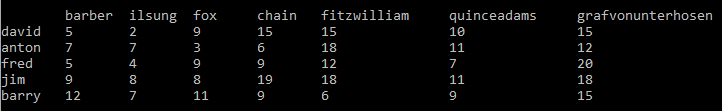
\includegraphics[scale=0.9]{q2-matrix}

\pagebreak\textbf{Problem 3}

We want to find 

$\argmax_{a, b, c} P(a\vert b)P(b\vert c)P(c) \\
= \argmax_{a}\argmax_{b}\argmax_{c} P(a\vert b)P(b\vert c)P(c) \\
= \argmax_{a}P(a\vert b)\argmax_{b}P(b\vert c)\argmax_{c} P(c)$

Let $\gamma(b) = \sum_c P(b\vert c)P(c)$ and $\gamma(a) = \sum_b P(a \vert b)\gamma(b)$

We get $\gamma(b = true) = 0.36$ and $\gamma(b = false) = 0.64$ with the following table:

\begin{table}[h]
	\begin{tabular}{|l|l|l|}
		\hline
		& b = true & b = false \\ \hline
		c = true  & 0.3      & 0.1       \\ \hline
		c = false & 0.06     & 0.54      \\ \hline
	\end{tabular}
\end{table}

Then, we get $\gamma(a = true) = 0.198$ and $\gamma(a = false) = 0.642$ with the following table:

\begin{table}[h]
	\begin{tabular}{|l|l|l|}
		\hline
		& a = true & a = false \\ \hline
		b = true  & 0.09      & 0.21       \\ \hline
		b = false & 0.108     & 0.432      \\ \hline
	\end{tabular}
\end{table}

As such, we see $\argmax_a \gamma(a)$ leads to \textbf{a = false}. After inspecting the 2nd table above, we see the value of b that contributes the most to $\gamma(a = false)$ is \textbf{b = false}, which is $\argmax_b P(a = true \vert b)\gamma(b)$.

Finally, we want $\argmax_c \gamma(b = false)$. When looking at the first table, the value of c that contributes the most to $\gamma(b = false)$ is when \textbf{c = false}.

So, using the max-product algorithm, through the use of backpointers, we have found argmax of the distribution occurs when \textbf{a = false, b = false, c = false}.

\pagebreak\textbf{Problem 4}

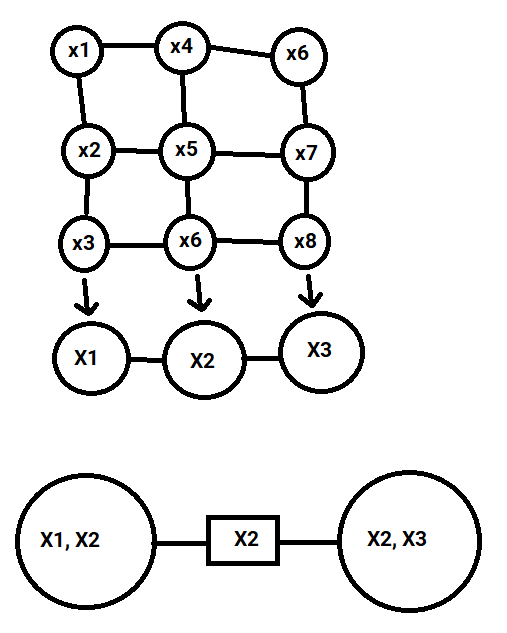
\includegraphics[scale=0.5]{q4}

The generated junction tree is shown in the above diagram where $\phi(X_1, X_2) = \phi(x_1, x_2, x_3, x_4, x_5, x_6)$ and $\phi(X_2, X_3) = \phi(x_4, x_5, x_6, x_7, x_8, x_9)$. Let 

$\phi(X_1, X_2) = \phi(x_1, x_2)\phi(x_2, x_3)\phi(x_1, x_4)\phi(x_2, x_5)\phi(x_3, x_6)\phi(x_4, x_5)\phi(x_5, x_6)$

$\phi(X_2, X_3) = \phi(x_4, x_7)\phi(x_5, x_8)\phi(x_6, x_9)\phi(x_7, x_8)\phi(x_8, x_9)$

$\phi(X_2) = 1$

We can now perform absorptions to calculate Z:

$\phi_1^*(X_2) = \sum_{X_1} \phi(X_1, X_2) = \sum_{x_1, x_2, x_3} = \phi(x_1, x_2)\phi(x_2, x_3)\phi(x_1, x_4)\phi(x_2, x_5)\phi(x_3, x_6)\phi(x_4, x_5)\phi(x_5, x_6)$

$\phi^*(X_2, X_3) = \phi(X_2, X_3)\frac{\phi_1^*(X_2)}{\phi(X_2)} = \phi(X_2, X_3)\phi^*(X_2) = \phi(X_2, X_3)\sum_{X_1} \phi(X_1, X_2)$

$\phi_2^*(X_3) = \sum_{X_2} \phi_1^*(X_2, X_3)$

$\phi^*(X_3, X_4) = \phi(X_3, X_4)\frac{\phi_2^*(X_3)}{\phi(X_3)}$

$\dots$

$\phi_{n-2}^*(X_{n-1}) = \sum_{X_{n-2}} \phi(X_{n-2}, X_{n-1})$

$\phi^*(X_{n-1}, X_n) = \phi(X_{n-1}, X_n)\frac{\phi_{n-2}^*(X_{n-1})}{\phi(X_{n-1})} = \phi(X_{n-1}, X_n)\sum_{X_{n-2}} \phi(X_{n-2}, X_{n-1})\dots \sum_{X_1} \phi(X_1, X_2)$\\

$Z = \sum_{X_{n-1}, X_n} \phi^*(X_{n-1}, X_n) \\
= \sum_{X_{n-1}, X_n} \phi(X_{n-1}, X_n)\sum_{X_{n-2}} \phi(X_{n-2}, X_{n-1}) \dots \sum_{X_2} \phi(X_2, X_3)\sum_{X_1} \phi(X_1, X_2)$

First, we must calculate the big X potentials $\phi(X_i, X_{i+1})$, not to be confused with little x potentials in the original lattice $\phi(x_i, x_{i+1})$. Since each $X_i$ stacks n variables (in an nxn lattice), it takes control of n binary variables. As such, it models $2^n$ possible variable configurations. In the JCT algorithm, since we have $\phi(X_i, X_{i+1})$, we must iterate over $2^n$ states for $X_i$ and $2_n$ states for $X_{i+1}$, for a total of $2^n(2^n) = 2^{2n}$ possible state configurations.

As shown above, for $\phi(X_1, X_2)$, for each state configuration, we must multiply N-1 nodes' vertical edge potentials, which is 2 in our case, then N nodes' horizontal edge potentials, which is N, and finally N-1 node's vertical edge potentials again. This leads to a total of (N-1) + N + (N-1) nodes used for multiplications, or 3N-3 multiplications in total. Then, to generalize this, notice how above $\phi(X_2, X_3)$ has fewer edge potentials than $\phi(X_1, X_2)$. This will be the case for all $\phi(X_i, X_{i+1})$ where $i \neq 1$. In this case, instead of 3n-3 multiplications across 3n-2 nodes, we will instead have 2n-2 multiplications across 2n-1 nodes. As such, to actually generate each pairwise big X edge potential, or in other words initialize them, we require $2^{2n}((3n-3) + (2n-2)) = 2^{2n}(5n-5)$ multiplications.

Now, when we actually want to compute Z, we first want to look at the right-most summation provided above, which is $\sum_{X_1} \phi(X_1, X_2)$. In this case, a new function will be generated such that $\phi_1^*(X_2) = \sum_{X_1} \phi(X_1, X_2)$. For this function, $X_2$ will have $2^n$ states, and the summation will sum across $2^n$ numbers, requiring $2^n - 1$ addition operations. As such, since each state requires $2^n-1$ additions, we get a total of $2^n(2^n-1) = 2^{2n} - 2^n$ operations to compute this function. All functions we will compute after this can be represented as $\phi_i^*(X_{i+1}) = \sum_{X_i} \phi(X_i, X_{i+1})\phi_{i-1}^*(X_i)$. In this case, there are still $2^n - 1$ additions and $2^n$ multiplications for each of the $2^n$ states. As such, to compute these subsequent functions, we require $2^n(2^n + (2^n - 1)) = 2^n(2^{n + 1} - 1) = 2^{2n+1} - 2^n$ calculations. We will have to perform these calculations for n-3 messages, all the way from $\phi_2^*(X_3)$ to $\phi_{n-2}^*(X_{n-1})$. Finally, when we eventually get to the final calculations of Z, we have to compute $\sum_{X_{n-1}, X_n} \phi(X_{n-1}, X_n)\phi_{n-2}^*(X_{n-1})$, which are the left-most values of that summation for Z as shown above. Since there is one multiplication per iteration of the loop, and the loop is iterating over two nodes with $2^n$ states each, there are a total of $2^n(2^n) = 2^{2n}$ loop iterations, leading to $2^{2n}$ multiplications, and it is easy to see there are $2^{2n} - 1$ additions, totaling $2^{2n} + (2^{2n} - 1) = 2^{2n + 1} - 1$ operations. As such, since $\phi_1^*(X_2)$ requires $2^{2n} - 2^n$ operations, $\phi_i^*(X_{i+1})$ requires $2^{2n+1} - 2^n$ for a total of n-3 functions, and $\sum_{X_{n-1}, X_n} \phi(X_{n-1}, X_n)\phi_{n-2}^*(X_{n-1})$ requires $2^{2n + 1} - 1$ operations, we get the following complexity for calculating Z:

$(2^{2n} - 2^n) + (n-3)(2^{2n+1} - 2^n) + (2^{2n+1} - 1)\\
= 2^{2n} - 2^n + n2^{2n+1} - n2^n - 3(2^{2n+1}) + 3(2^n) + 2^{2n+1} - 1\\
= n2^{2n+1} - 3(2^{2n+1}) + 2^{2n+1} + 2^{2n} - 2^n - n2^n + 3(2^n) - 1\\
= 2^{2n+1}(n - 3 + 1) + 2^{2n} - 2^n(1 + n - 3) - 1\\
= 2^{2n+1}(n - 2) + 2^{2n} - 2^n(n - 2) - 1\\
= (n-2)(2^{2n+1} - 2^n) + 2^{2n} - 1$

For n = 10, we have \textbf{log(Z) = 186.7916}.

\pagebreak\textbf{Problem 5}

a) The symptom marginals can be found below:

\begin{table}[h!]
	\begin{tabular}{|l|l|l|l|}
		\hline
		i  & $p(s_i = 1)$ & i & $p(s_i = 1)$ \\ \hline
		1  & 0.4418 & 21 & 0.7613 \\ \hline
		2  & 0.4567 & 22 & 0.6956 \\ \hline
		3  & 0.4414 & 23 & 0.5087 \\ \hline
		4  & 0.4913 & 24 & 0.4200 \\ \hline
		5  & 0.4939 & 25 & 0.3519 \\ \hline
		6  & 0.6575 & 26 & 0.3896 \\ \hline
		7  & 0.5046 & 27 & 0.3260 \\ \hline
		8  & 0.2687 & 28 & 0.4696 \\ \hline
		9  & 0.6491 & 29 & 0.5229 \\ \hline
		10 & 0.4907 & 30 & 0.7173 \\ \hline
		11 & 0.4226 & 31 & 0.5242 \\ \hline
		12 & 0.4291 & 32 & 0.3537 \\ \hline
		13 & 0.5450 & 33 & 0.5127 \\ \hline
		14 & 0.6330 & 34 & 0.5294 \\ \hline
		15 & 0.4295 & 35 & 0.3858 \\ \hline
		16 & 0.4588 & 36 & 0.4891 \\ \hline
		17 & 0.4276 & 37 & 0.6336 \\ \hline
		18 & 0.4043 & 38 & 0.5896 \\ \hline
		19 & 0.5821 & 39 & 0.4232 \\ \hline
		20 & 0.5896 & 40 & 0.5282 \\ \hline
	\end{tabular}
\end{table}

b) Instead of using the JCT algorithm, we can use the following:

$P(s_i) \\
= \sum_{s\backslash s_i}\sum_{d_1\dots d_20} P(s_1, \dots, s_{40}, d_1, \dots, d_{20}) \\
=  \sum_{s\backslash s_i}\sum_{d_1\dots d_20} P(s_1 \vert Pa(s_1))\dots P(s_{40} \vert Pa(s_{40}))\prod_{j = 1}^{20} P(d_j) \\
= \sum_{d_1\dots d_{20}} P(s_i \vert Pa(s_i))\prod_{j = 1}^{20} P(d_j) \\
= \sum_{Pa(s_i)} P(s_i \vert Pa(s_i))P(Pa_1(s_i))P(Pa_2(s_i))P(Pa_3(s_i)) \\$

In the above equations, $s_i$ is the i-th symptom, $d_j$ is the j-th disease, and $Pa_i(s_i)$ is the i-th parent disease of $s_i$. For each $s_i$, there are 3 parent diseases. For example, if the parents of $s_4$ are $d_2, d_8, d_{22}$, then the above probability evaluates to \\$P(s_4) = \sum_{d_2, d_8, d_{22}} P(s_4 \vert d_2, d_8, d_{22})P(d_2)P(d_8)P(d_{22})$.

After implementing this method, it can be seen the max difference between the two sets of probabilities is 3.153e-14.

\pagebreak c) After setting $s_1, \dots, s_5 = 1$ and $s_6, \dots, s_{10} = 2$, we compute the marginals of the diseases as follows:

\begin{table}[h]
	\begin{tabular}{|l|l|l|l|}
		\hline
		j  & $p(d_j = 1)$ & j & $p(d_j = 1)$ \\ \hline
		1  & 0.0298 & 11 & 0.2873 \\ \hline
		2  & 0.3181 & 12 & 0.4898 \\ \hline
		3  & 0.9542 & 13 & 0.8996 \\ \hline
		4  & 0.3966 & 14 & 0.6196 \\ \hline
		5  & 0.4965 & 15 & 0.9205 \\ \hline
		6  & 0.4352 & 16 & 0.7061 \\ \hline
		7  & 0.1875 & 17 & 0.2012 \\ \hline
		8  & 0.7012 & 18 & 0.9085 \\ \hline
		9  & 0.0431 & 19 & 0.8650 \\ \hline
		10 & 0.6103 & 20 & 0.8839 \\ \hline
	\end{tabular}
\end{table}

\pagebreak\textbf{Problem 6}

a) The junction tree is as follows:

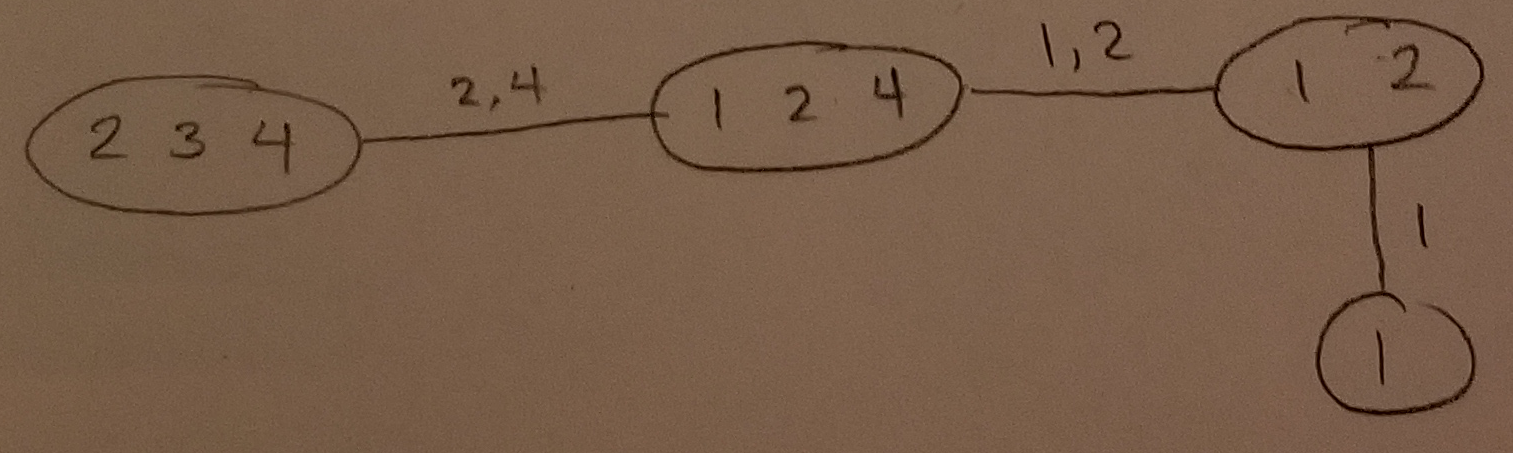
\includegraphics[scale=0.4]{q6-junctiontree}

b) The normal way to calculate the marginal is as follows:

$P(x_1, x_2, x_3, x_4)\\
= \sum_{x_2}\sum_{x_3}\sum_{x_4}\phi(x_1, x_2)\phi(x_2, x_3)\phi(x_3, x_4)\phi(x_4, x_1)\\
= \sum_{x_2}\sum_{x_4}\phi(x_1, x_2)\phi(x_4, x_1)\sum_{x_3}\phi(x_2, x_3)\phi(x_3, x_4)\\
= \sum_{x_2}\sum_{x_4}\phi(x_1, x_2)\phi(x_4, x_1)\phi_{x_3}(x_2, x_4)\\
= \sum_{x_2}\phi(x_1, x_2)\sum_{x_4}\phi(x_4, x_1)\phi_{x_3}(x_2, x_4)\\
= \sum_{x_2}\phi(x_1, x_2)\phi_{x_4}(x_1, x_2)\\
= \phi_{x_2}(x_1)$

Now, through the absorption procedure, we get the following:

Let $\phi(x_1, x_2, x_4) = \phi(x_1, x_2)\phi(x_4, x_1)$, $\phi(x_2, x_3, x_4) = \phi(x_2, x_3)\phi(x_3, x_4)$, and $\phi(x_2, x_4) = 1$.

$\phi_1^*(x_2, x_4) = \sum_{x_3}\phi(x_2, x_3, x_4)$

$\phi^*(x_1, x_2, x_4) = \phi(x_1, x_2, x_4)\frac{\phi_1^*(x_2, x_4)}{\phi(x_2, x_4)} = \phi(x_1, x_2, x_4)\frac{\sum_{x_3}\phi(x_2, x_3, x_4)}{\phi(x_2, x_4)} = \phi(x_1, x_2, x_4)\sum_{x_3}\phi(x_2, x_3, x_4) = P(x_1, x_2, x_4)$

$\phi_2^*(x_1, x_2) = \sum_{x_4} \phi^*(x_1, x_2, x_4)$

$\phi^*(x_1, x_2) = \phi(x_1, x_2)\frac{\phi_2^*(x_1, x_2)}{\phi(x_1, x_2)}$

$\phi_3^*(x_1) = \sum_{x_2}\phi^*(x_1, x_2)$

$\phi^*(x_1) = \phi(x_1)\frac{\phi_3^*(x_1)}{\phi(x_1)} = \phi_3^*(x_1)$

As such,w e have computed the marginal of $x_1$. To verify it is the correct result, we will expand the marginal below:

$\phi^*(x_1) \\
= \phi_3^*(x_1) \\
= \sum_{x_2}\phi^*(x_1, x_2) \\
= \sum_{x_2}\phi(x_1, x_2)\frac{\phi_2^*(x_1, x_2)}{\phi(x_1, x_2)} \\
= \sum_{x_2}\frac{\phi(x_1, x_2)}{\phi(x_1, x_2)}\sum_{x_4} \phi^*(x_1, x_2, x_4)\\
= \sum_{x_2}\frac{\phi(x_1, x_2)}{\phi(x_1, x_2)}\sum_{x_4} \phi(x_1, x_2, x_4)\frac{\phi_1^*(x_2, x_4)}{\phi(x_2, x_4)}\\
= \sum_{x_2}\frac{\phi(x_1, x_2)}{\phi(x_1, x_2)}\sum_{x_4} \phi(x_1, x_2, x_4)\frac{\sum_{x_3}\phi(x_2, x_3, x_4)}{\phi(x_2, x_4)}\\
= \sum_{x_2}\sum_{x_3}\sum_{x_4}\frac{\phi(x_1, x_2)}{\phi(x_1, x_2)} \phi(x_1, x_2, x_4)\phi(x_2, x_3, x_4)\frac{1}{\phi(x_2, x_4)}\\
= \sum_{x_2}\sum_{x_3}\sum_{x_4}\frac{\phi(x_1, x_2)}{\phi(x_1, x_2)} \phi(x_1, x_2)\phi(x_4, x_1)\phi(x_2, x_3)\phi(x_3, x_4)\frac{1}{\phi(x_2, x_4)}\\
= \sum_{x_2}\sum_{x_3}\sum_{x_4} \phi(x_1, x_2)\phi(x_4, x_1)\phi(x_2, x_3)\phi(x_3, x_4)\\
= \sum_{x_2}\sum_{x_3}\sum_{x_4} \phi(x_1, x_2)\phi(x_2, x_3)\phi(x_3, x_4)\phi(x_4, x_1)$

This above equation is the exact same equation we got above while we were solving for the marginal of $x_1$. As such, we can safely confirm the absorption gives us the correct result.

\pagebreak\textbf{Problem 7}

a) 

The following diagram shows (a) the bayesian network modeling the joint distribution, (b) the bayesian network creating a fully-connected network after moralization, and (c) the junction tree:

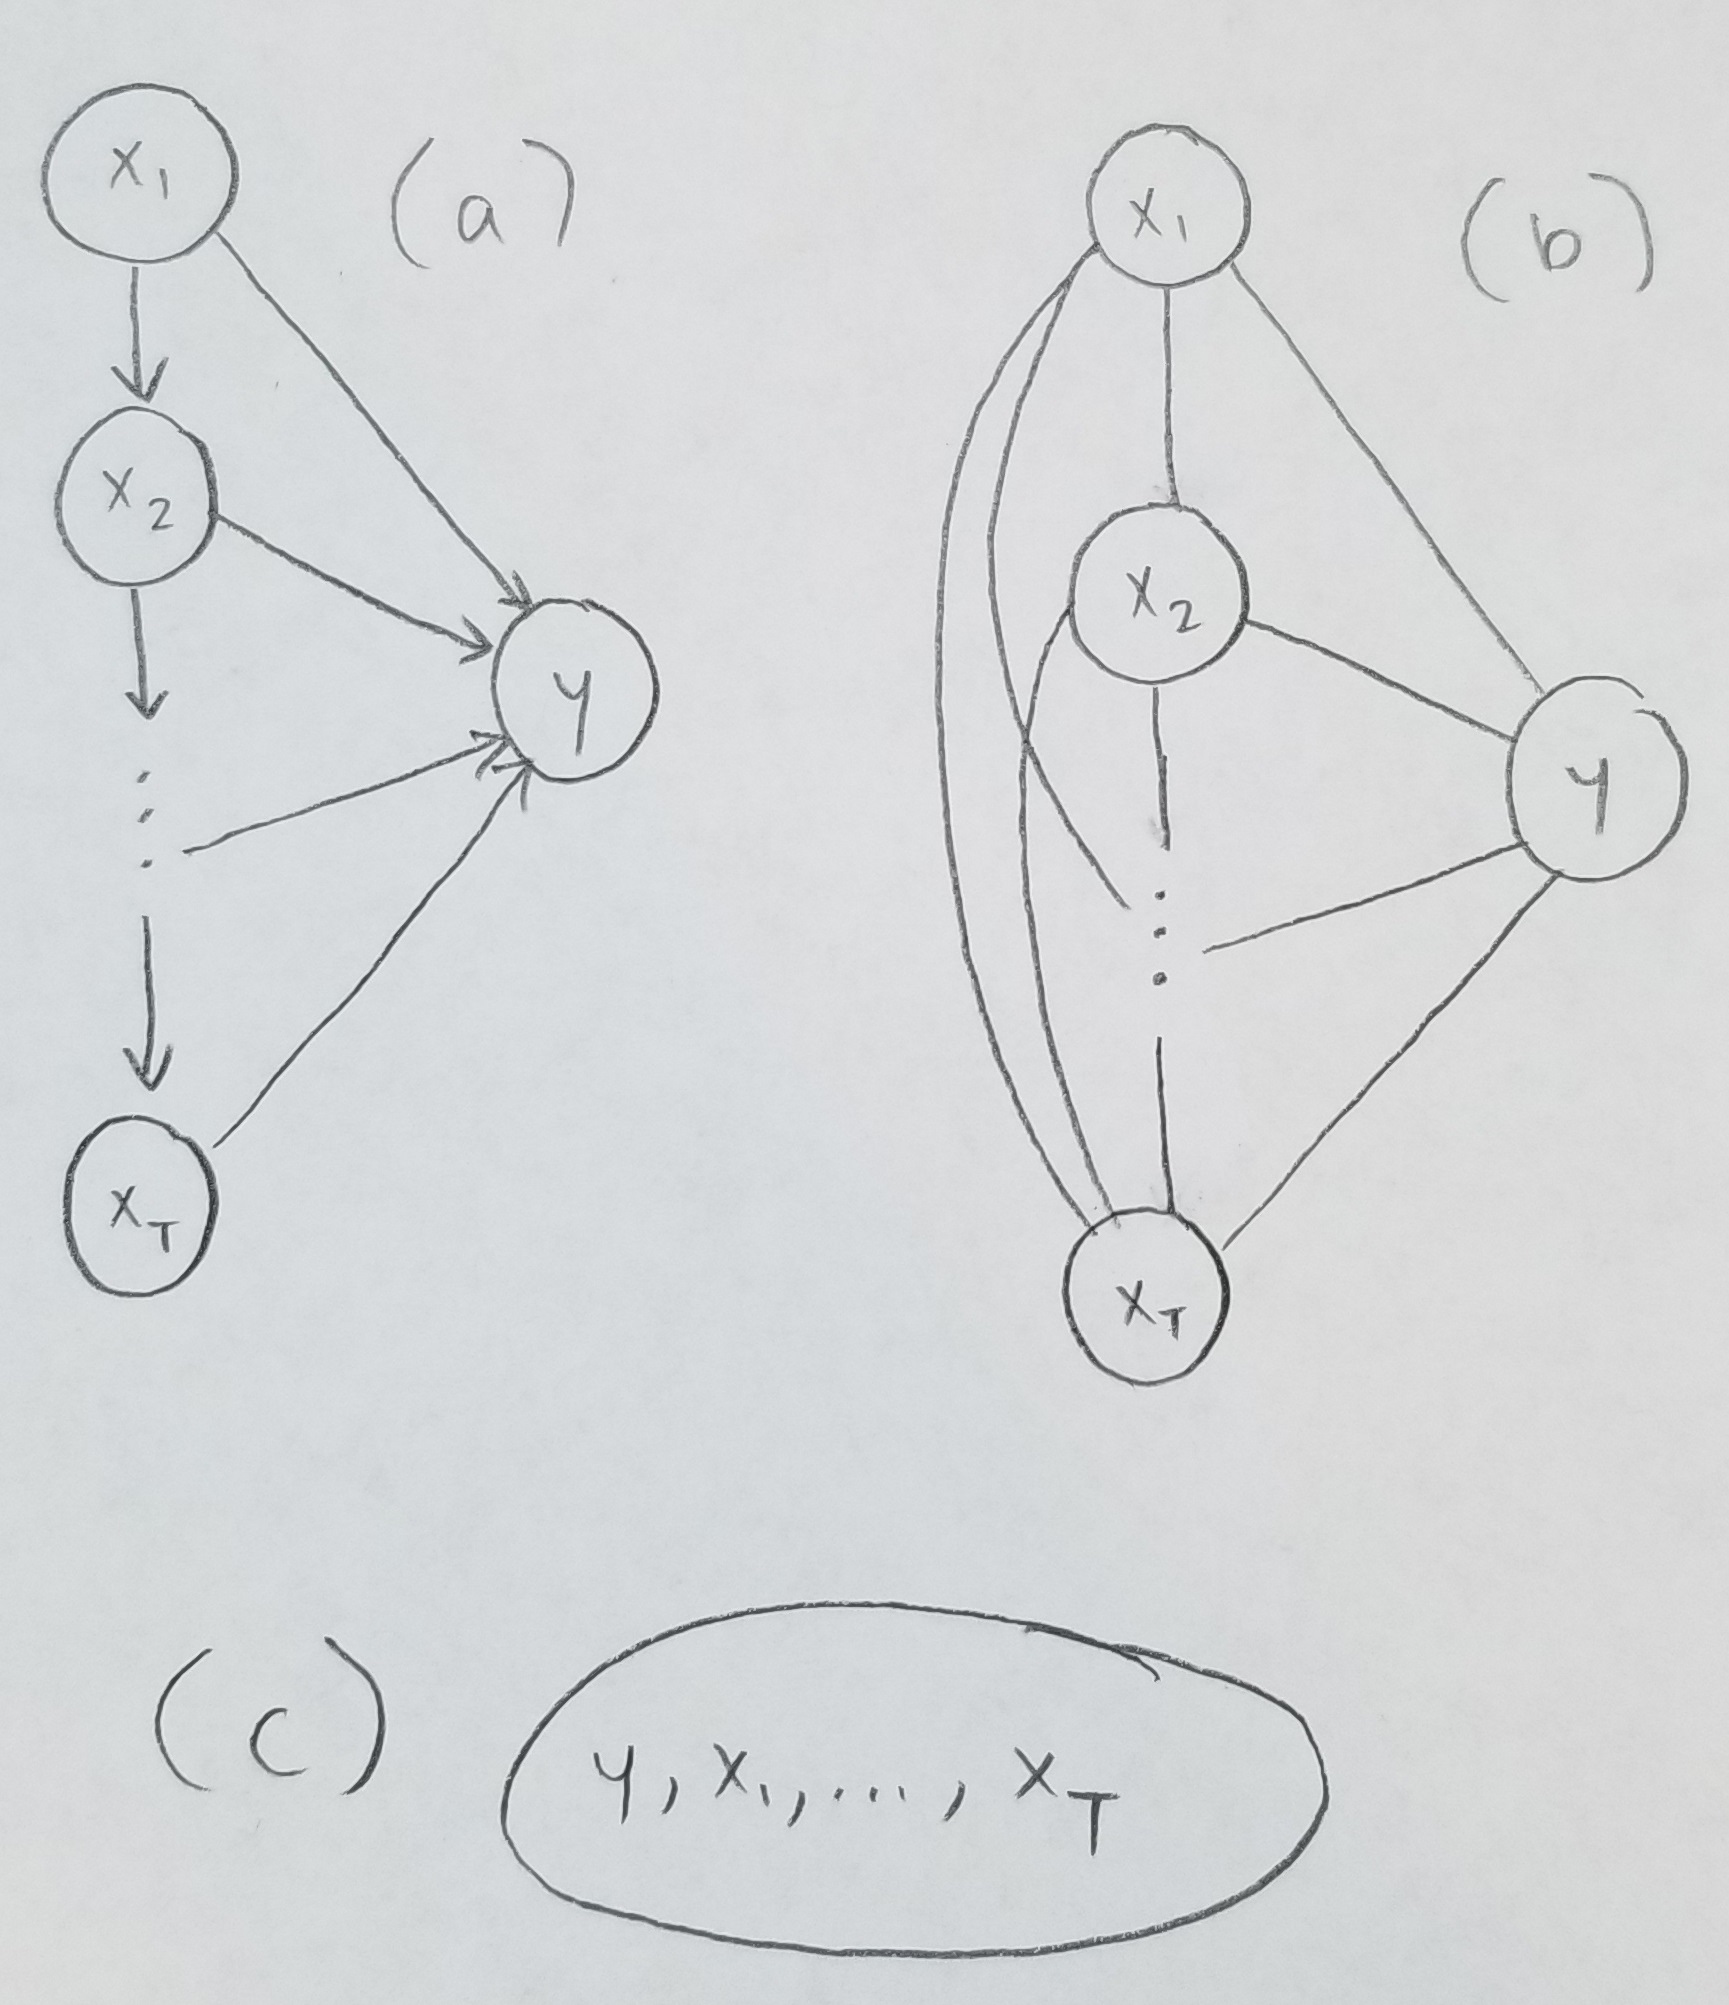
\includegraphics[scale=0.1]{q7-trees}

We want to figure out the runtime complexity of calculating $p(x_T)$ as given by the junction tree algorithm. The junction tree algorithm requires the moralization step. In moralization, two parents of a node must have a direct connection. As such, since all nodes are parents of y, all nodes must be connected to each other, leading to a fully-connected network. Since the network becomes fully-connected after moralization, the junction tree algorithm will give us one huge node containing all nodes in the graph, which is represented as $\phi(y, x_1, \dots, x_T) = p(y \vert x_1, \dots, x_T)p(x_1)\prod_{t = 2}^{T} p(x_t \vert x_{t-1})$. Since all variables are binary, and there are $T+1$ nodes, there are a total of $2^{T+1}$ possible state configurations for this node potential. However, since we want just the potential for $x_T$, we only need to marginalize, or sum, over $T$ nodes, leading to $2^T-1$ additions for each of the two states of $x_T$. Since there are 2 states for $x_T$ and we require $2^T - 1$ additions per state, we require $2(2^T - 1) = 2^{T+1} - 1$ calculations, or $O(2^T)$ time for the junction tree algorithm.

b)

We can reduce this time complexity significantly through variable elimination, as seen below:

$p(x_T) \\
= \sum_{y, x_1, \dots, x_{T-1}} p(y \vert x_1, \dots, x_T)p(x_1)\prod_{t = 2}^{T} p(x_t \vert x_{t-1}) \\
= \sum_{x_1, \dots, x_{T-1}} p(x_1)\prod_{t = 2}^{T} p(x_t \vert x_{t-1}) \sum_y p(y \vert x_1, \dots, x_T)$

We know $\sum_y p(y \vert x_1, \dots, x_T) = 1$.

$= \sum_{x_1, \dots, x_{T-1}} p(x_1)\prod_{t = 2}^{T} p(x_t \vert x_{t-1}) \\
= \sum_{x_1, \dots, x_{T-1}} p(x_1)p(x_2 \vert x_1)\dots p(x_{T-1})p(x_T)$

Let $\varphi_{x_i}(x_{i+1}) = \sum_{x_i} \varphi_{x_{i-1}}(x_i)p(x_{i+1} \vert x_i)$, with a special casing being $\varphi_{x_1} = \sum_{x_1} p(x_1)p(x_{2} \vert x_1)$

$= \sum_{x_2, \dots, x_{T-1}} \varphi_{x_1}(x_2)p(x_3 \vert x_2)\dots p(x_{T-1})p(x_T) \\
= \sum_{x_3, \dots, x_{T-1}} \varphi_{x_2}(x_3)p(x_4 \vert x_3)\dots p(x_{T-1})p(x_T) \\
= \sum_{x_{T-1}} \varphi_{x_{T-2}}(x_{T-1})p(x_T \vert x_{T-1}) \\
= \varphi_{x_{T-1}}(x_{T})$

Each function $\varphi_{x_i}(x_{i+1})$ has two states, and it sums over 2 values, requiring 1 multiplication for each summation. As such, for each state, there are 2 multiplications and 1 addition, totalling $2(2 + 1) = 6$ calculations to compute $\varphi_{x_i}(x_{i+1})$. Since we create $T-1$ of these tables, a total of $6(T-1)$ calculations are required to create all the tables. As such, with this new runtime of $6(T-1) = 6T - 6 = O(T)$, we can see this alternative algorithm is linear in complexity.

\pagebreak\textbf{Problem 8}

a) 

We eliminate the variables in the order $x_{10}$, $x_{9}$, $x_{7}$, $x_{6}$, $x_{5}$, $x_{4}$, $x_{3}$, $x_{2}$, $x_0$ as follows:

$p(x_1 \vert x_{11}, x_8) \\
= \sum_{x_0, x_2, x_3, x_4, x_5, x_6, x_7, x_9, x_{10}} \phi(x_0, x_1, x_2)\phi(x_0, x_2, x_3)\phi(x_0, x_3, x_4)\phi(x_1, x_2, x_3)\phi(x_1, x_3, x_4)\\\phi(x_2, x_3, x_4)\prod_{i = 5}^{11}\phi(x_1, x_2, x_i)\phi(x_1, x_3, x_i)\phi(x_1, x_4, x_i)\phi(x_2, x_3, x_i)\phi(x_2, x_4, x_i)\phi(x_3, x_4, x_i)$

Let $\varphi_{11}(x_1, x_2, x_3, x_4) = \phi(x_1, x_2, x_{11})\phi(x_1, x_3, x_{11})\phi(x_1, x_4, x_{11})\phi(x_2, x_3, x_{11})\phi(x_2, x_4, x_{11})\phi(x_3, x_4, x_{11})$

Note: $x_{11}$ is a given variable, so we do not need to sum over its values.

$= \sum_{x_0, x_2, x_3, x_4, x_5, x_6, x_7, x_9, x_{10}} \phi(x_0, x_1, x_2)\phi(x_0, x_2, x_3)\phi(x_0, x_3, x_4)\phi(x_1, x_2, x_3)\phi(x_1, x_3, x_4)\\\phi(x_2, x_3, x_4)\varphi_{11}(x_1, x_2, x_3, x_4)\prod_{i = 5}^{10}\phi(x_1, x_2, x_i)\phi(x_1, x_3, x_i)\phi(x_1, x_4, x_i)\\\phi(x_2, x_3, x_i)\phi(x_2, x_4, x_i)\phi(x_3, x_4, x_i)$

Let $\varphi_{10}(x_1, x_2, x_3, x_4) = \sum_{x_{10}} \phi(x_1, x_2, x_{10})\phi(x_1, x_3, x_{10})\phi(x_1, x_4, x_{10})\phi(x_2, x_3, x_{10})\phi(x_2, x_4, x_{10})\phi(x_3, x_4, x_{10})$

$= \sum_{x_0, x_2, x_3, x_4, x_5, x_6, x_7, x_9} \phi(x_0, x_1, x_2)\phi(x_0, x_2, x_3)\phi(x_0, x_3, x_4)\phi(x_1, x_2, x_3)\phi(x_1, x_3, x_4)\\\phi(x_2, x_3, x_4)\varphi_{10}(x_1, x_2, x_3, x_4)\varphi_{11}(x_1, x_2, x_3, x_4)\prod_{i = 5}^{9}\phi(x_1, x_2, x_i)\phi(x_1, x_3, x_i)\phi(x_1, x_4, x_i)\\\phi(x_2, x_3, x_i)\phi(x_2, x_4, x_i)\phi(x_3, x_4, x_i)$

Let $\forall_{i \in \{5, 6, 7, 9\}}\varphi_{i}(x_1, x_2, x_3, x_4) = \sum_{x_{i}} \phi(x_1, x_2, x_{i})\phi(x_1, x_3, x_{i})\phi(x_1, x_4, x_{i})\phi(x_2, x_3, x_{i})\\\phi(x_2, x_4, x_{i})\phi(x_3, x_4, x_{i})$

And $\varphi_{8}(x_1, x_2, x_3, x_4) =  \phi(x_1, x_2, x_{8})\phi(x_1, x_3, x_{8})\phi(x_1, x_4, x_{8})\phi(x_2, x_3, x_{8})\phi(x_2, x_4, x_{8})\phi(x_3, x_4, x_{8})$ for a similar reason to $x_{11}$ mentioned above.

$= \sum_{x_0, x_2, x_3, x_4} \phi(x_0, x_1, x_2)\phi(x_0, x_2, x_3)\phi(x_0, x_3, x_4)\phi(x_1, x_2, x_3)\phi(x_1, x_3, x_4)\\\phi(x_2, x_3, x_4)\prod_{i = 5}^{11}\varphi_{i}(x_1, x_2, x_3, x_4)$

Let $\varphi_4(x_0, x_1, x_2, x_3) = \sum_{x_4} \phi(x_0, x_3, x_4)\phi(x_1, x_3, x_4)\phi(x_2, x_3, x_4)\prod_{i = 5}^{11}\varphi_i(x_1, x_2, x_3, x_4)$

$= \sum_{x_0, x_2, x_3} \phi(x_0, x_1, x_2)\phi(x_0, x_2, x_3)\phi(x_1, x_2, x_3)\varphi_4(x_0, x_1, x_2, x_3)$

Let $\varphi_3(x_0, x_1, x_2) = \sum_{x_3} \phi(x_0, x_2, x_3)\phi(x_1, x_2, x_3)\varphi_4(x_0, x_1, x_2, x_3)$

$= \sum_{x_0, x_2} \phi(x_0, x_1, x_2)\varphi_3(x_0, x_1, x_2)$

Let $\varphi_2(x_0, x_1) = \sum_{x_2} \phi(x_0, x_1, x_2)\varphi_3(x_0, x_1, x_2)$

$= \sum_{x_0} \varphi_2(x_0, x_1)$

Let $\varphi_0(x_1) = \sum_{x_0} \varphi_2(x_0, x_1)$

$= \varphi_0(x_1)$

Now, we will calculate the runtime of this algorithm. $\varphi_{11}$ and $\varphi_8$ require 5 simple multiplications each. Then, $\forall_{i \in \{5, 6, 7, 9, 10\}}\varphi_{i}(x_1, x_2, x_3, x_4)$ requires 5 multiplications for both iterations of the loop, in addition to 1 addition, resulting in 2(5) + 1 = 11 operations. For $\varphi_4(x_0, x_1, x_2, x_3)$, there are 9 multiplications for each iteration, and one addition, resulting in 2(9) + 1 = 19 operations. For $\varphi_3(x_0, x_1, x_2)$ requires 2 multiplications for each iteration, and one addition, resulting in 2(2) + 1 = 5 calculations. For $\varphi_2(x_0, x_1)$, we require there is one multiplication per loop iteration, and one addition, resulting in 2(1) + 1 = 3 calculations. Finally, $\varphi_0(x_1)$ requires 1 addition. So, the total number of calculations is 2(5) + 5(11) + 19 + 5 + 3 + 1 = 93 computations.

In terms of space, we need $2^4 = 16$ storage spaces for $\forall_{i \in \{5, \dots, 11\}}\varphi_{i}(x_1, x_2, x_3, x_4)$, $2^4 = 16$ storage space for $\varphi_4(x_0, x_1, x_2, x_3)$, $2^3 = 8$ storage spaces for $\varphi_3(x_0, x_1, x_2)$, $2^2 = 4$ spaces for $\varphi_2(x_0, x_1)$, and 2 spaces for $\varphi_0(x_1)$. In total, this means we need 7(16) + 16 + 8 + 4 + 2 = 142 storage spaces for this variable elimination algorithm.

b) The messages here correspond to the marginal distribution over the four main factors (labeled 1, 2, 3, and 4), which are HasFlu, HasFoodPoisoning, HasHayFever, and HasPneumonia. So, basically, the messages being passed through the network correspond to the probabilities of diseases.
\end{document}
